\documentclass{iopconfser}

\usepackage{float}
\usepackage{graphicx}
\usepackage{subcaption}
\usepackage[automake]{glossaries-extra}
\usepackage{ragged2e}

% \makeglossaries

\setabbreviationstyle[acronym]{long-postshort-user}
\glssetcategoryattribute{acronym}{nohyperfirst}{true}
\setabbreviationstyle{short-nolong}
\makeglossaries

% --------------------
% ---- Glossaries ----
% --------------------
\newglossaryentry{asyncio}{name=Asyncio, description={A Python library for asynchronous code.}}
\newglossaryentry{stim}{name=STIM300, description={A MEMS-based \gls{imu}}}
\newglossaryentry{f9p}{name=F9P, description={A Global Navigation Satellite System (GNSS) receiver manufactured by u-blox.}}

% --------------------
% ----- Acronyms -----
% --------------------
\newacronym{asv}{ASV}{Autonomous Surface Vehicle}
\newacronym{dolp}{DoLP}{Degree of Linear Polarization}
\newacronym{aolp}{AoLP}{Angle of Linear Polarization}
\newacronym{sitaw}{SITAW}{Situational Awareness}
\newacronym{poe}{PoE}{Power over Ethernet}
\newacronym{pps}{PPS}{Pulse Per Second}
\newacronym{cpfa}{CPFA}{Color-Polarization Filter Array}
\newacronym{utc}{UTC}{Coordinated Universal Time}
\newacronym{imu}{IMU}{Inertial Measurement Unit}
\newacronym{tov}{TOV}{Time of Validity}
\newacronym{tm2}{TM2}{Time mark data}
\newacronym{gnss}{GNSS}{Global Navigation Satellite System}
\newacronym{ptp}{PTP}{Precision Time Protocol}

% \glsaddall
% \makenoidxglossaries

% \glsunset{cpu}
\glsunset{gnss}
\glsunset{imu}
\glsunset{tm2}
\glsunset{utc}

% --------------------
% ----- Shortcuts ----
% --------------------


\begin{document}

\title{A Lightweight, Polarization-Camera Equipped Sensor Rig for the Development of Autonomous Surface Vehicles}

\author{Emil Martens$^{1}$, Edmund Førland Brekke$^{1}$, Rudolf Mester$^{2}$, Annette Stahl$^{1}$}

\affil{$^1$Department of Engineering Cybernetics, NTNU, Trondheim, Norway}

\affil{$^2$Department of Computer Science, NTNU, Trondheim, Norway}

\email{emil.martens@ntnu.no}

\begin{abstract}
    \justifying 
    \gls{sitaw} of \glsps{asv} is critical for safe and efficient maritime operations, enabling these vehicles to better understand their environment and make informed decisions.
    High-quality data sets from relevant maritime environments are needed to advance the development of \gls{sitaw}, as it is both the backbone of any learning-based method as well as the development and validation of classical methods.
    Research vessels like the full-scale ferry \textit{milliAmpere2} provide such data, but there tends to be a considerable labor cost associated with their operation, and they are not always available on demand.
    To address these challenges, a stand-alone lightweight sensor rig has been developed to facilitate the collection of high-quality data sets and to showcase the potential of polarization cameras in the maritime domain.
    The sensor rig is designed for easy transport and operation by a single individual or for temporary attachment to any existing vessel, making it versatile for a wide range of data collection scenarios.
    It is equipped with a Jetson Orin AGX computer, two dual-band GNSS receivers, a high-grade IMU, and two polarization cameras.
    Emphasis has been put on precisely synchronizing all devices using a microcontroller and a custom Linux kernel configuration supporting \gls{pps} synchronization.
    Stereo polarization video is collected, preprocessed, and compressed in real-time using CUDA C++ and GStreamer. This makes it possible to preview the video feeds wirelessly through a custom web-based GUI from a nearby phone or computer.
    
    To demonstrate the potential of the sensor rig and the benefit of polarization cameras in the maritime domain, we present a new data set from the river Nidelva in Trondheim, Norway. 
    We show how the new information from the polarization cameras can be used to remove sun glare and improve water surface segmentation by leveraging the physical properties of the polarization of water reflections.
    This new data set consists of synchronized stereo polarization video, raw IMU data, and raw GNSS data and will be made publically available to the research community with the conference.
    
    
\end{abstract}
\pagebreak
\begin{figure}[H]
    \centering
    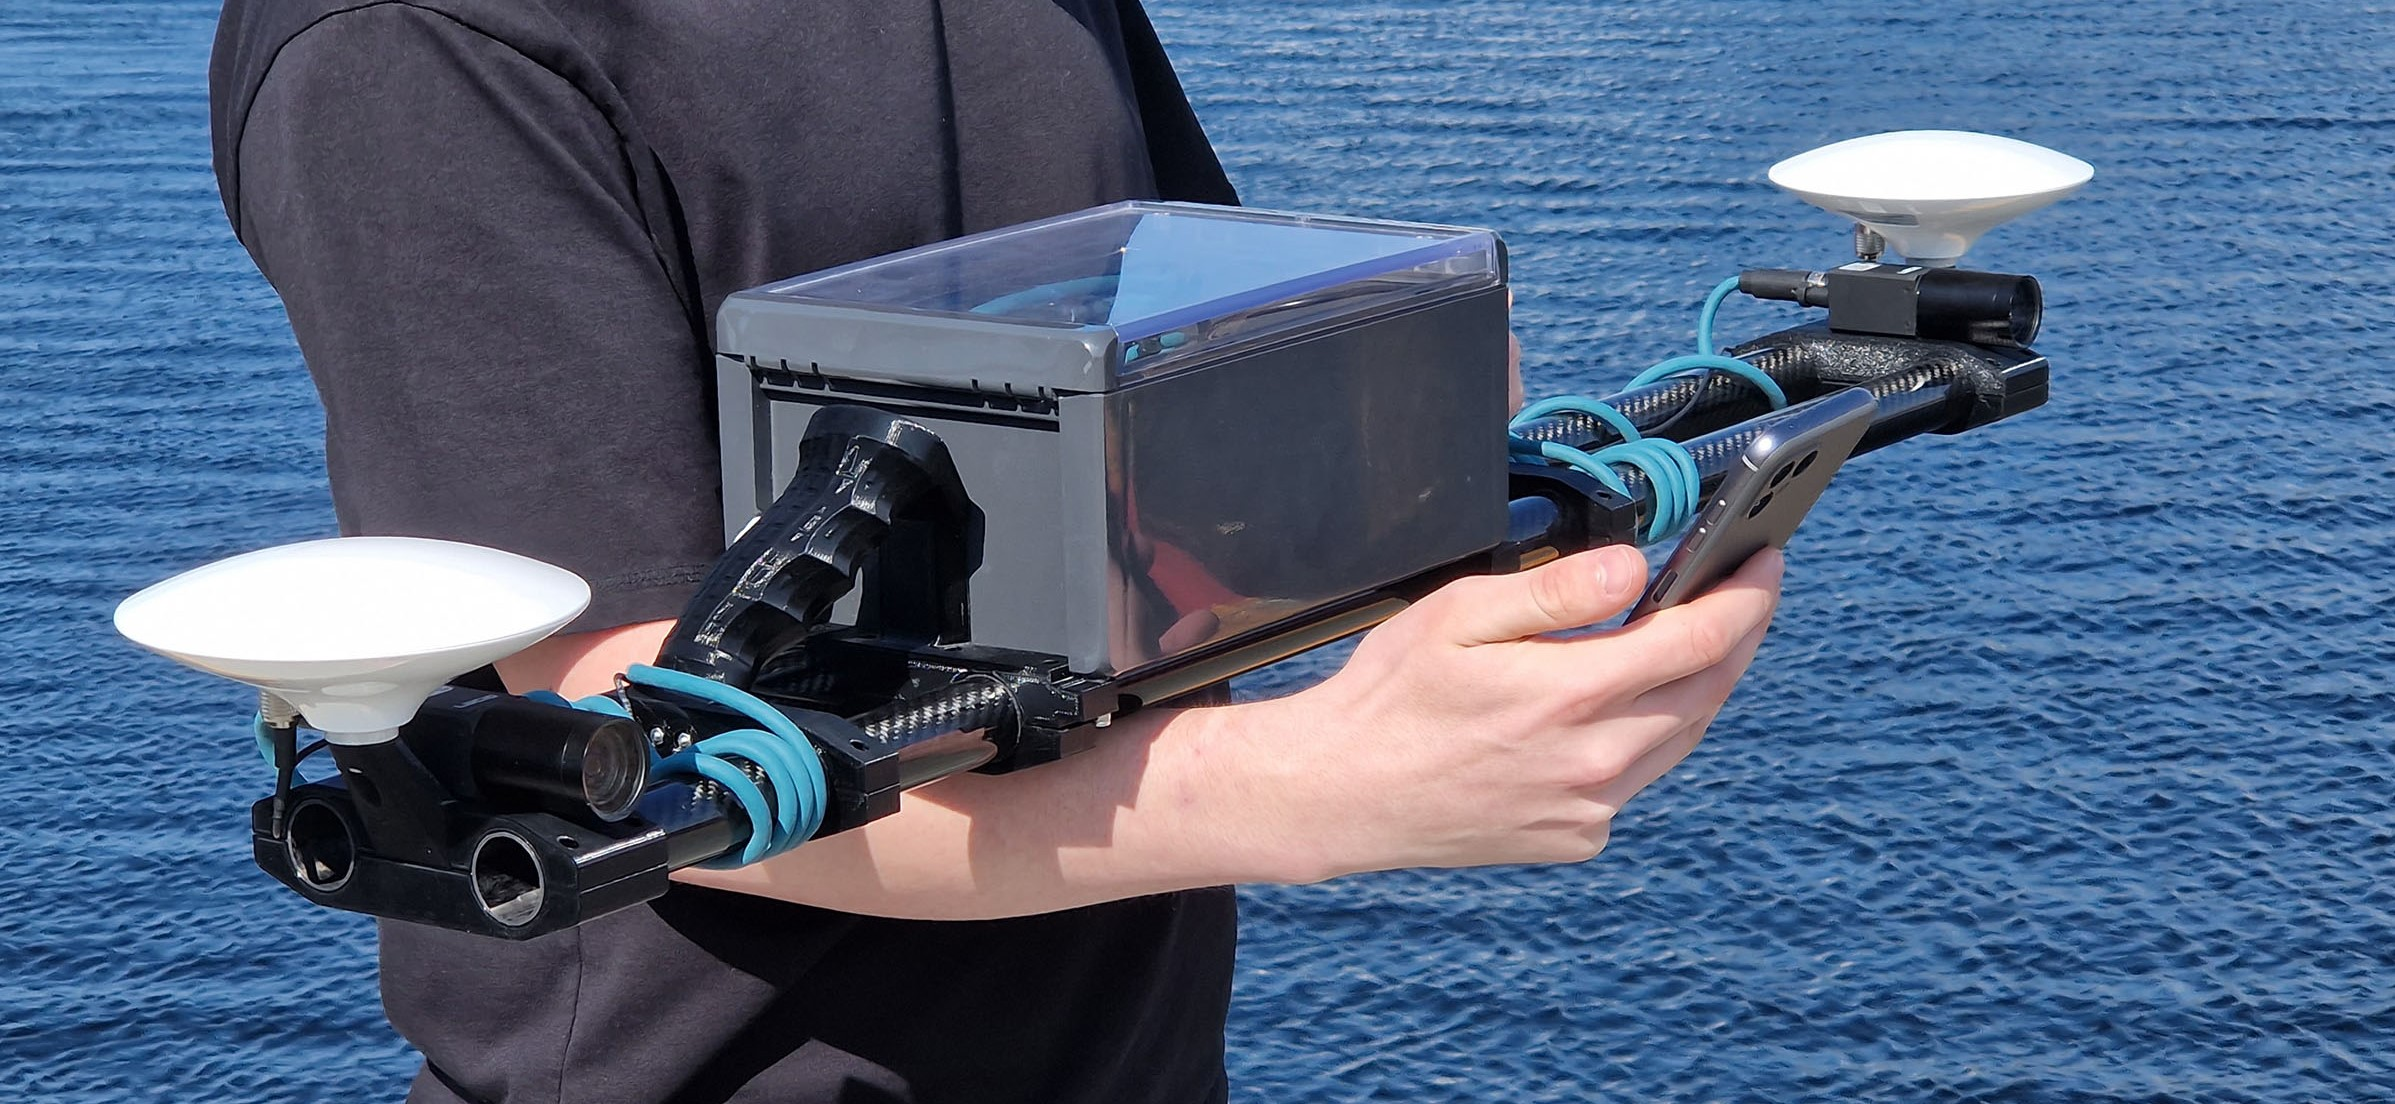
\includegraphics[width=0.9\textwidth]{figures/operation.jpg}
    \caption{Human operation of the sensor rig. Ergonomic handles ensure comfort and the operator can control and monitor the acquisition through a phone over the phone's mobile hotspot.}
\end{figure}


\begin{figure}[H]
    % \centering
    \subcaptionbox{Scene as observed by a regular camera.}{
        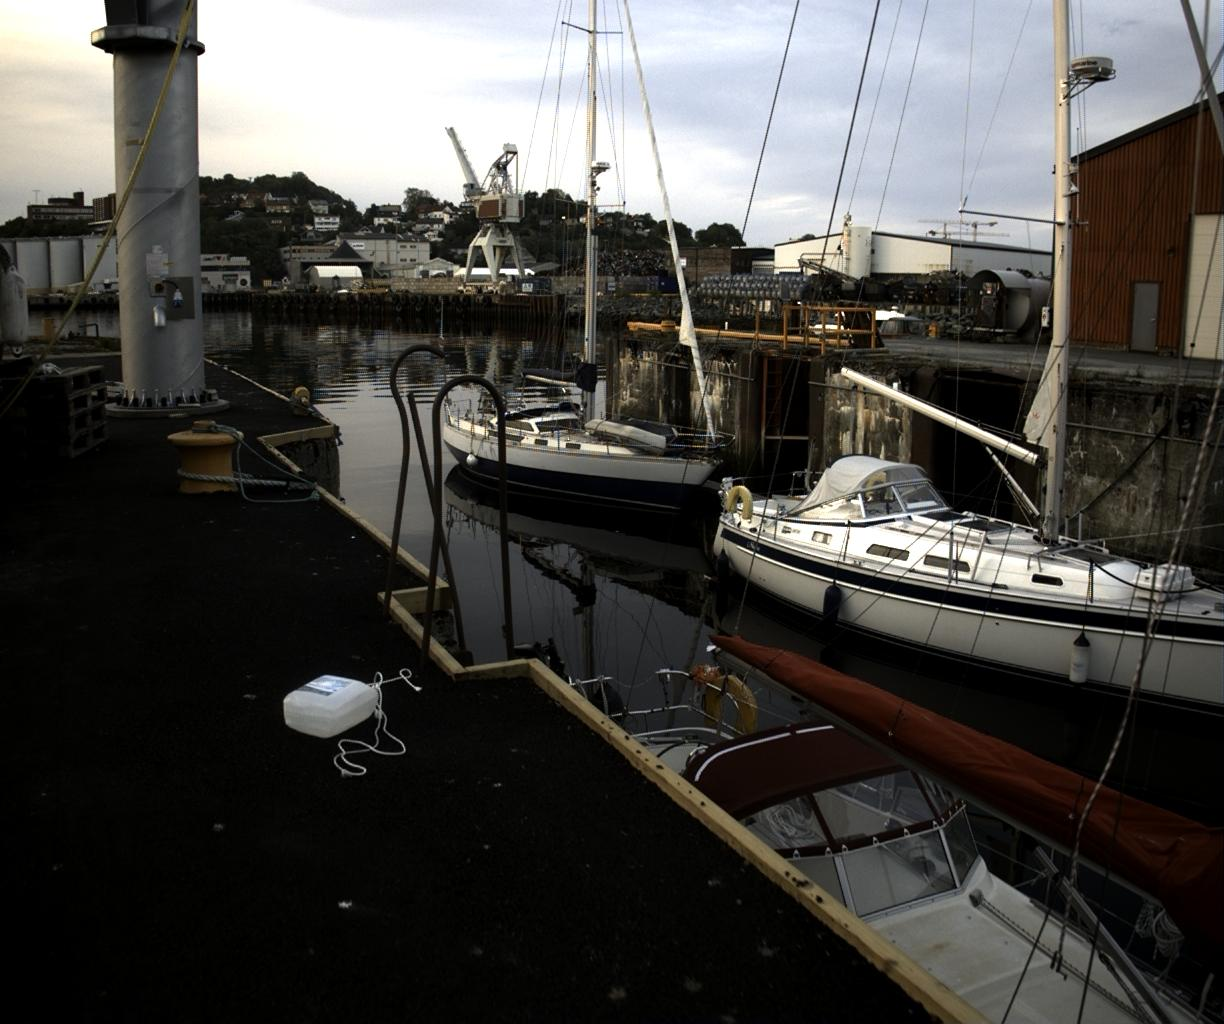
\includegraphics[width=0.48\textwidth]{figures/regular_right_96.jpeg}
    }
    \hfill
    \subcaptionbox{Visualization of raw polarization data with \glsentrylong{aolp} and \glsentrylong{dolp} visualized as hue and value of an HSV image.}{
        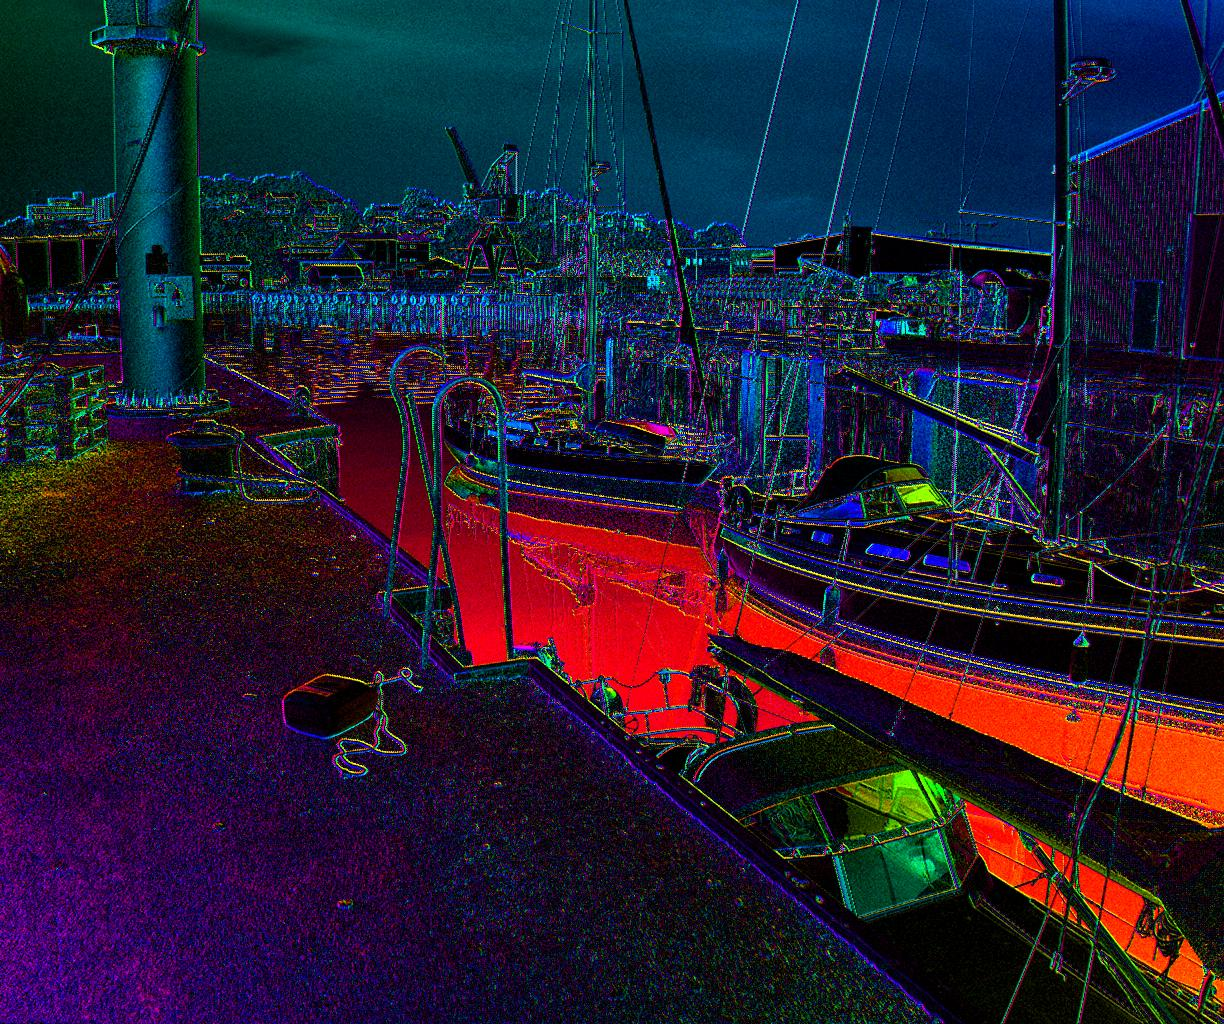
\includegraphics[width=0.48\textwidth]{figures/aolp_right_96.jpeg}
    }
    \caption{Illustration of how polarization cameras provide additional information in a maritime context.}
    \label{fig:polarization_visualization}
\end{figure}


\end{document}